\documentclass[utf8, diplomski]{fer}
\usepackage{booktabs}
\usepackage{longtable}
\usepackage{ltablex}
\usepackage{pdfpages}
\usepackage[hidelinks]{hyperref}
\usepackage{mathtools}
\usepackage{listings}
\usepackage{subfig}
\setcitestyle{numbers,square,super}
\usepackage[export]{adjustbox}
\usepackage{float}
\usepackage{tabularx}
\usepackage{enumitem}
\usepackage{mathrsfs}


\begin{document}

\thesisnumber{2231}

\title{Obrana dubokih konvolucijskih modela od neprijateljskih primjera}

\author{Matej Dobrovodski}

\maketitle

\iffalse \includepdf[pages=-]{img/content/izvornik.pdf} \fi

\tableofcontents

\chapter{Uvod}
\section{Raspoznavanje objekata}
Raspoznavanje objekata jedan je od ključnih problema područja računalnog vida. Pri rješavanju problema raspoznavanja objekata se na ulaz nekog sustava dovede slika nekog objekta, a na izlazu se očekuje ispravna klasifikacija u neki od predodređenih razreda. Čovjeku ovaj zadatak ne predstavlja veliki problem, no još uvijek ne postoji zadovoljavajuće rješenje problema koje bi vrijedilo za opći slučaj. Trenutno najbolja takva rješenja temelje se na konvolucijskim neuronskim mrežama. \par
Razvoj konvolucijskih mreža počeo je osamdesetih godina prošlog stoljeća. Počelo je razvojem \textit{neocognitron}[citat?]-a--neuronske mreže inspirirane biološkim stanicama vidne kore mozga. Krajem devedesetih godina se pojavljuje konvolucijska neuronska mreža LeNet5. LeNet5 mreža je vrlo uspješno raspoznavala rukom pisane znamenke te je ova mreža bila početna točka za daljnja istraživanja drugih neuronskih mreža. [citati] \par
\textit{ImageNet}[citat] projekt je velika baza podataka predviđena za istraživanje područja raspoznavanja objekata. S više od $14$ milijuna slika podijeljenih u $20000$ kategorija, \textit{ImageNet} skup je daleko najveći slobodno dostupni skup. Počevši od 2010.[?] godine, \textit{ImageNet} projekt organizira godišnje natjecanje, \textit{ImageNet Large Scale Visual Recognition Challenge} (ILSVRC). Veliki skok u točnosti pri raspoznavanju dogodio se 2012. godine kada je konvolucijska neuronska mreža \textit{AlexNet}[citat] postigla top-5 pogrešku od samo $15.3\%$, što je bilo $10.8\%$ manje od sljedeće mreže. To je postignuto korištenjem grafičkih procesora pri treniranju, što je potaknulo svojevrsnu revoluciju u području dubokog učenja. \par
Do 2017. godine, većina timova u natjecanju je imala top-5 točnost veću od $95\%$. Danas se u raznim bibliotekama mogu naći unaprijed istrenirane mreže koje postižu vrlo dobre rezultate, te će se one spominjati i koristiti u nastavku rada. Neke od tih mreža su primjerice \textit{ResNet}[citat], \textit{Xception}[citat] i \textit{VGG}[citat]. Sve spomenute mreže postižu vrlo zadovoljavajuće točnosti pri ispitivanju (top-5 točnosti iznad $90\%$) i čini se da mogu dobro generalizirati. No u nastavku rada će biti pokazan oblik napada na konvolucijske mreže koji dovodi u pitanje činjenicu da današnje konvolucijske mreže dobro generaliziraju.
\section{Neprijateljski primjeri}
Krajem $2013.$ godine pojavljuje se prvi izravni "napad" na duboke neuronske mreže\citep{Szegedy2014IntriguingPO}, gdje je jedna od meta bila prethodno spomenuta uspješna mreža \textit{AlexNet}. Polazna pretpostavka je da duboki modeli, usprkos tome što dobro generaliziraju, imaju ugrađene svojevrsne \textit{slijepe pjege} koje se isplati istražiti.
\par
Vrijedi da za neki ispravno klasificirani ulaz $x$ postoji područje $x + r$ u blizini ulaza te je uobičajeno da modeli ulazne vrijednosti iz tog područja također ispravno klasificiraju, isto kao i $x$. U općem slučaju vrijedi da neprimjetne perturbacije iz tog područja (npr. nasumični šum slabog intenziteta) ne mijenjaju izlaz modela. To je pretpostavka lokalne generalizacije i tipično vrijedi za probleme iz područja računalnog vida.
\par
Međutim, ispostavilo se da ta pretpostavka lokalne generalizacije zapravo ne vrijedi. Otkriveno je da je moguće konstruirati perturbaciju $r$ koja dovodi do pogrešne klasifikacije, a ljudskom oku nije uočljiva. Takve slike se nazivaju neprijateljskim primjerima, a taj pojam se može generalizirati i na mnoga druga područja i na sličan način se mogu napasti sustavi pretvaranja teksta u govor, sustavi za detekciju zloćudnih programa i praktički svi sustavi koji se oslanjaju na dosadašnje modela za duboko učenje. 
\par
Ono što je iznenađujuće i što je potaklo daljnje istraživanje je to što je zapravo iznimno lako za pronaći takve neprijateljske primjere na \textit{state of the art} modelima kod kojih je perturbacija $r$ potpuno neprimjetna i to što nije nimalo očito zašto mreže neispravno klasificiraju takve ulaze. Jedan od originalnih napada je prikazan na slici \ref{fig:alexnet_adv} gdje \textit{AlexNet} mreža predviđa da su novonastale slike zapravo slike noja.

\begin{figure}[H]
\centering
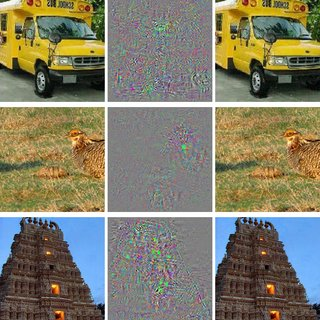
\includegraphics[width=0.5\textwidth,keepaspectratio]{img/other/alexnet_adv.jpg}
\caption{Primjer suparničkog napada na \textit{AlexNet} mrežu\citep{Szegedy2014IntriguingPO}. U lijevom stupcu su originalne, ispravno klasificirane slike. U srednjem stupcu se nalazi perturbacija koja se nadodaje na originalnu sliku, a u desnom stupcu su sve tri novonastale slike klasificirane kao noj.}
\label{fig:alexnet_adv}
\end{figure}

U radu je dan pregled nekoliko metoda generiranja neprijateljskih primjera: neke metode su prikazane zbog njihove povijesne važnosti i utjecaja na daljni razvoj metoda, dok su neke metode iznimno snažne i mjerilo za uspješnost obrane od suparničkih napada. Pokazano je i koliko su napadi uspješni protiv poznatih mreža te kako niti jedan od široko dostupnih modela nije unaprijed otporan na napade. Uz napade su pokazane i obrane, s naglaskom na njihovu (ne)uspješnost pri odupiranju od postojećih suparničkih napada, probleme koji su gotovo svim obranama zajednički te potencijalnu budućnost razvoja uspješnijih obrana. 


\chapter{Programska potpora}
\section{Odabir biblioteke za duboko učenje}
Postoji mnogo biblioteka koje pružaju sve potrebno za duboko učenje i računalni vid. U nastavku rada se koristi \textit{Tensorflow} 2\citep{abadi2016tensorflow} u kombinaciji s bibliotekom \textit{Keras}\citep{chollet2015keras}. Zbog ogromnog dobitka u brzini izvođenja, ove biblioteke su korištene zajedno s platformom \textit{CUDA} koja omogućava iskorištavanje grafičkog procesora za obradu opće namjene (eng. \textit{graphics processing unit for general purpose processing}, GPGPU). Grafička kartica korištena u sklopu generiranja rezultata u radu je NVIDIA GeForce RTX 2060 SUPER.
\section{Biblioteke za neprijateljske primjere}
Usprkos tome što su suparnički primjeri relativno nov koncept, već postoji mnogo biblioteka koje pružaju implementaciju velikog broja suparničkih napada, a često su i napadi implementirani izravno od strane autora napada. Istaknule su se tri biblioteke za generiranje suparničkih napada: \textit{CleverHans}\citep{papernot2018cleverhans}, \textit{Foolbox Native}\citep{rauber2017foolbox} i \textit{Adversarial Robustness Toolbox (ART)}\citep{art2018}.
\par
Za odabir biblioteke je razmatrano nekoliko stvari: dostupnost i ekstenzivnost dokumentacije, raznovrsnost implementiranih napada, jednostavnost korištenja, zahtjevana programska potpora te postoji li implementacija obrana. Za svaku biblioteku je implementirano generiranje neprijateljskih primjera napadom koji je opisan u \ref{fgm}, a napad je proveden na model opisan u .
\par
\textit{Cleverhans} ima kratku dokumentaciju za sve napade i poveznicu na relevantni rad koji opisuje napad, međutim ne postoji dokumentacija u formatu koji se lako pretražuje. \textit{Foolbox} i \textit{ART} imaju dokumentaciju dostupnu u takvom formatu, međutim \textit{Foolbox} dokumentacija ne opisuje kako se napad poziva i s kojim argumentima, što otežava korištenje bez detaljnijeg proučavanja izvornog kôda, dok je \textit{ART} dokumentacija eksplicitna kod toga.
\par
Što se tiče jednostavnosti korištenja, \textit{Cleverhans} je bio najjednostavniji za primjenu u ovom jednostavnom primjeru. \textit{Foolbox} zahtjeva da se slike pretvore u određen format prije pokretanja napada, što otežava korištenje. \textit{ART}, međutim, zahtjeva dodatne informacije pri konstruiranju napada kao što su broj razreda, dimenzije ulaza, funkcija gubitka i granične vrijednosti, što druge biblioteke ne traže.
\par
\textit{Cleverhans} i \textit{Foolbox} imaju vrlo specifične zahtjeve za programsku potporu, iako će \textit{Cleverhans} u budućnosti podupirati više od samo \textit{Tensorflow}. \textit{ART} pruža potporu za mnoštvo biblioteka: \textit{Tensorflow} (v1 i v2), \textit{Keras}, \textit{PyTorch}, \textit{MXNet} i još njih.
\par
Od navedenih biblioteka, \textit{ART} je jedina koja već sada ima implementirane neke od obrana u literaturi. \textit{Cleverhans} biblioteka ima planove za implementaciju u budućnosti, dok \textit{Foolbox} podržava samo napade.
\par
Zbog svega navedenog, u nastavku rada se koristi samo \textit{Adversarial Robustness Toolbox}. Dodatno, autori biblioteke su vrlo aktivni na \textit{GitHub}-u i iznimno brzo reagiraju kada se postavi pitanje ili prijavi problem. Pri izradi rada otkriveno je nekoliko \textit{bug}-ova koji su popravljeni u vrlo kratkom roku te su zahvaljujući autorima minimalno usporavali izradu rada.

\section{Skupovi podataka}
\textit{ImageNet}\citep{?} je široko korištena baza podataka slika s preko $14$ milijuna slika raspoređenih u više od $20000$ razreda. \textit{ImageNet} je praktički postao standard za treniranje i evaluaciju rada modela pri klasifikaciji objekata. Neki od modela korišteni u radu su unaprijed trenirani na \textit{ImageNet} bazi podataka na kojima postižu iznimno visoku točnost.
\par
Neke obrane i posljedično napadi će u nastavku rada biti evaluirani na \textit{CIFAR-10}\citep{?} skupu podataka. \textit{CIFAR-10} sadrži samo $10$ disjunktnih razreda, te $50000$ slika za treniranje mreže. Nužno je koristiti i ovaj skup podataka jer pojedine obrane još uvijek nije moguće skalirati na \textit{ImageNet} razinu jer vrijeme izvođenja nije razumno.
\par
U svrhu rada je također odabrano $16$ slika koje bi \textit{ImageNet} modeli trebali ispravno klasificirati. Popis slika i izlazi određenih modela nalaze se u dodatku\textsuperscript{\ref{dodatak}}.
\section{Konvolucijski modeli}
Primarna meta napada u radu je mreža \textit{ResNet V2}\citep{resnetv2}, i to verzija s 50 slojeva koja je unaprijed trenirana na \textit{ImageNet} skupu. Mreža postiže top-1 točnost od $76\%$, te top-5 točnost od $93\%$.  U početnim fazama izrade rada razmatrano je više mreža, međutim \textit{ResNet} mreža je puno brža pri evaluaciji što ubržava i olakšava evaluaciju napada i obrana. Korištenje ove mreže ne smanjuje općenitost ideja predstavljenih u radu, pošto su sve konvolucijske mreže jednako ranjive na neprijateljske napade. Lakoća provođenja neprijateljskih napada je "problem" koji sve konvolucijske mreže dijele u jednakoj mjeri, i trenutno ne postoji niti jedna takva mreža koja je sama po sebi otporna na njih. Dodatno, kôd priložen uz rad dopušta provođenje napada na sljedeće mreže: \textit{DenseNet121}, \textit{VGG16}, \textit{VGG19}, \textit{MobileNetV2} te \textit{Xception}.
\par
Osim \textit{ResNet} mreže, dodatno je konstruirana i jednostavna konvolucijska mreža za klasifikaciju \textit{CIFAR-10} slika. Mreža se sastoji od 11 slojeva, redom:
\begin{enumerate}[noitemsep, label=\textbullet]
  \item konvolucijski sloj oblika $32\times32\times32$ s filtrom veličine $3\times3$
  \item konvolucijski sloj oblika $32\times32\times32$ s filtrom veličine $3\times3$
  \item sloj sažimanja oblika $2\times2$
  \item sloj ispadanja s vjerojatnošću $0.25$
  \item konvolucijski sloj oblika $16\times162\times64$ s filtrom veličine $3\times3$
  \item konvolucijski sloj oblika $16\times162\times64$ s filtrom veličine $3\times3$
  \item sloj sažimanja oblika $2\times2$
  \item sloj ispadanja s vjerojatnošću $0.25$
  \item potpuno povezani sloj veličine $512$
  \item sloj ispadnja s vjerojatnošću $0.50$
  \item potpuno povezani sloj veličine $10$, pošto se klasificra u 10 razreda
\end{enumerate}

\begin{figure}[H]
\centering
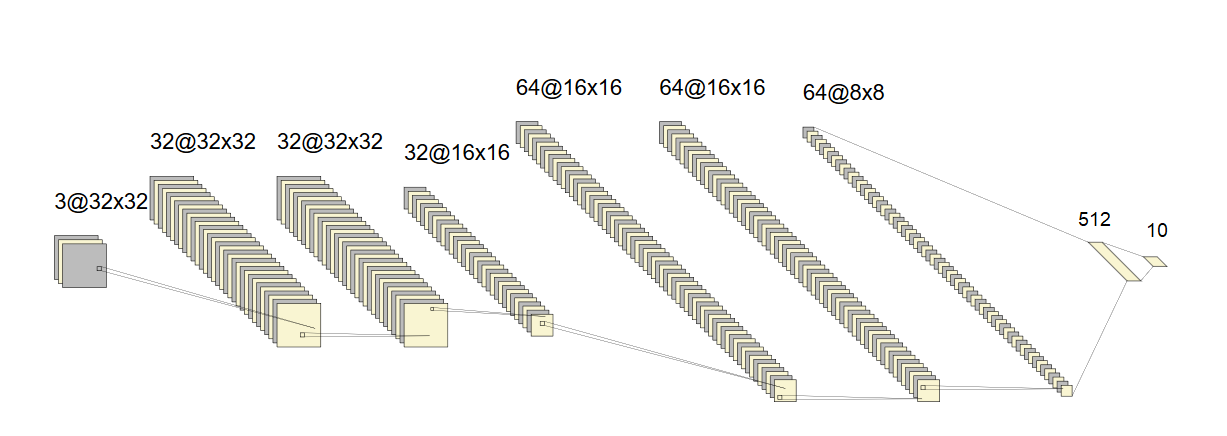
\includegraphics[width=1\textwidth,keepaspectratio]{img/other/toy_cifar10.png}
\caption{Skica jednostavne mreže za \textit{CIFAR-10} mrežu. Nisu prikazani slojevi ispadanja.}
\label{fig:toy_cifar10}
\end{figure}

Ukupno mreža ima $2,168,362$ parametara koji se mogu naučiti. Na slici \ref{fig:toy_cifar10} je skica mreže. Aktivacijska funkcija između relevantnih slojeva je \textit{ReLU}. Mreža već nakon $15$ epoha lako postiže točnost od $75\%$ na skupu za testiranje korištenjem stohastičnog gradijentnog spusta uz stopu učenja od $0.02$, bez ikakvog dodatnog podešavanja hiperparametara. Nakon $25$ epoha postiže točnost od $79.47\%$, no i u tom trenutku mreža nije pretrenirana. Za potrebe rada nije nužno maksimizirati točnost jer ne bi promijenilo rezultate. Jednako je lagano za pronaći suparničke primjere i na vrlo dobro istreniranim mrežama kao i ovakvim jednostavnim mrežama.


\chapter{Neprijateljski primjeri I}
\section{Model prijetnje}
Model prijetnje (eng. \textit{threat model}) je proces kojim se potencijalne prijetnje mogu nabrojati i identificirati te se mogu odrediti određene mjere kao prioritet. Neki od dijelova modela prijetnje mogu biti: frekvencija interakcije s metom napada, željena vrsta pogrešne klasifikacije, količina znanja o meti napada i specifičnost napada. Prije opisivanja navedenih aspekata modela prijetnje uvedeno je nekoliko relevantnih simbola koji se učestalo pojavljuju u literaturi i u ovom radu.

\textbf{Osnovni pojmovi i simboli} \\
\begin{tabular}{ l c l }
\textbullet \ $f(\cdot)$ & -- & model dubokog učenja \\ 
\textbullet \ $x$, $l$ & -- & originalni ulaz te pripadajuća labela \\  
\textbullet \ $x'$, $l'$ & -- & neprijateljski primjer i pripadajuća labela \\
\textbullet \ $J(\cdot)$ & -- & funkcija gubitka, u većini slučajeva gubitak unakrsne entropije \\
\textbullet \ $||\cdot||_{p}$ & -- & p-norma, p je najčešće $0$, $2$ ili $\infty$. Dodatna korištena oznaka za norme je $\ell_{p}$.
\end{tabular}
\linebreak
\linebreak

\begin{table}[H]
\textbf{Frekvencija interakcije s metom napada}
\begin{tabularx}{\textwidth}{ l c X }
\textbullet \ Jednokratni napad & -- & jednokratni napadi (eng. \textit{one-time}) su napadi kojima je potreban samo jedan pristup modelu da generiraju neprijateljski primjer. Ovi napadi su brzi, ali i mnogo slabiji od iterativnih napada te nisu u fokusu istraživanja. Na primjer, napad opisan u \ref{fgm} je jednokratni napad. \\ 
\textbullet \ Iterativni napad & -- & iterativni napadi zahtjevaju više pristupa modelu da bi generirali neprijateljski primjer. Ovakvi napadi generiraju daleko bolje neprijateljske primjere. Većina napada pripada ovoj kategoriji.
\end{tabularx}
\end{table}

\begin{table}[H]
\textbf{Vrsta pogrešne klasifikacije}
\begin{tabularx}{\textwidth}{ l c X }
\textbullet \ Lažno pozitivni napad & -- & lažno pozitivni (eng. \textit{false positive}) primjeri u kontekstu neprijateljskih napada kod klasifikacijskih problema su čovjeku potpuno neprepoznatljivi (npr. šum), dok mreža s visokom vjerojatnošću klasificira sliku. \\ 
\textbullet \ Lažno negativni napad & -- & lažno negativni (eng. \textit{false negative}) primjeri su oni koje čovjek vrlo lako prepozna, a mreža pogrešno klasificira zbog nevidljive perturbacije. Fokus rada su od početka lažno negativni primjeri. Usporedba napada dana je u slici \ref{fig:fp_fn}.
\end{tabularx}
\end{table}


\begin{figure}[H]
  \centering
  \subfloat[Lažno pozitivni napad. Mreža klasificra sliku kao prostirka za molitvu (eng. \textit{prayer rug}) s vjerojatnošću $98.66\%$.]{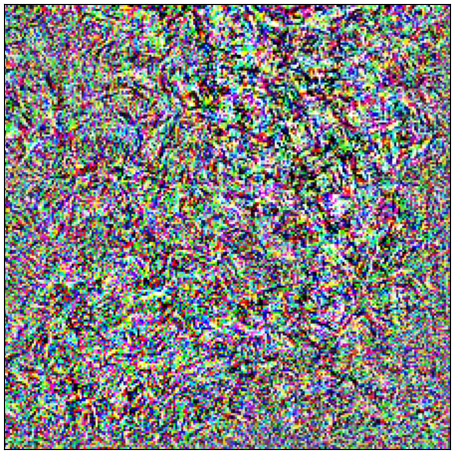
\includegraphics[width=0.48\textwidth]{img/results/prayer_rug_98-66_resnet_cw.png}\label{fig:a}}
  \hfill
  \subfloat[Lažno negativni napad. Mreža klasificra sliku kao zmaj (eng. \textit{kite}) s vjerojatnošću $91.89\%$.]{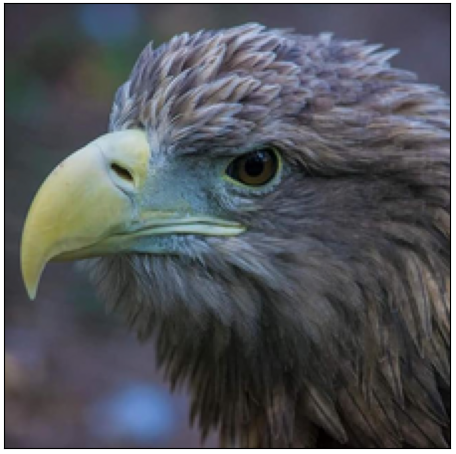
\includegraphics[width=0.48\textwidth]{img/results/kite_91-89_resnet_cw.png}\label{fig:b}}
  \caption{Primjeri lažno pozitivnog i lažno negativnog napada. Napad proveden na \textit{ResNet50V2} mreži korištenjem \textit{Carlini and Wagner} $\ell_{2}$ napada opisanog u \ref{x}.}
\end{figure}\label{fig:fp_fn}


\begin{table}[H]
\textbf{Znanje o meti napada}
\begin{tabularx}{\textwidth}{ l c X }
\textbullet \ Bijela kutija & -- & model se naziva bijela kutija (eng. \textit{white box}) ako je sve o modelu unaprijed poznato napadaču, uključujući: arhitekturu, parametre mreže, aktivacijske funkcije, hiperparametre i sve druge moguće detalje mreže. Napadi koji se temelje na modelu bijele kutije često iskorištavaju gradijente mreže pri konstruiranju neprijateljskog primjera. \\ 
\textbullet \ Crna kutija & -- & suprotno tome, model crne kutije (eng. \textit{black box}) pretpostavlja nedostatak svih mogućih informacija, osim izlaza iz mreže. Na primjer, ukoliko se napada neka mreža "u oblaku", njoj se pristupa tako da joj se preda ulaz te nije moguće direktno saznati dodatne detalje o mreži. Začudo, moguće je konstruirati neprijateljske primjere samo na temelju izlaza mreže.
\end{tabularx}
\end{table}

\begin{table}[H]
\textbf{Specifičnost napada}
\begin{tabularx}{\textwidth}{ l c X }
\textbullet \ Ciljani napad & -- & ciljani napad (eng. \textit{targeted attack}) je oblik napada gdje se za neki neprijateljski primjer pokušava dobiti unaprijed određen izlaz mreže. Uz to, dodatni zahtjev može biti i da se maksimizira vjerojatnost odabranog razreda. \\ 
\textbullet \ Neciljani napad & -- & neciljani napad (eng. \textit{untargeted attack}) zahtjeva jedino da je klasifikacija neprijateljskog primjera neispravna. Općenito je lakše i brže konstruirati neciljani napad.
\end{tabularx}
\end{table}

\section{Pojava prvih neprijateljskih primjera}
U uvodu je opisana osnovna ideja neprijateljskih primjera iz jednog od najranijih radova na temu neprijateljskih primjera\citep{Szegedy2014IntriguingPO}, a u nastavku je ideja dodatno razrađena i ukratko opisana optimizacijska metoda generiranja suparničkih primjera.
\par
Implicitno je pretpostavljeno da mreže imaju svojstvo lokalne generalizacije. Za neki dovoljno mali radijus $\epsilon > 0$ u blizini ulaza $x$ (epsilon okolina), postoji ulaz $x + r$ takav da je $||r|| < \epsilon$ koji će također imati veliku vjerojatnost pripadanja ispravnom klasifikacijskom razredu na izlazu mreže. Slabo vidljive promjene u pravilu ne mijenjaju drastično izlaz mreže, što se može i pokazati dodavanjem šuma na neku ulaznu sliku. Dapače, neke mreže su nasumičnom deformacijom ulaza pri treniranju povećavale robusnost modela. Pokazalo se da svojstvo lokalne generalizacije zapravo u velikoj mjeri nije prisutno kod tadašnjih (a i današnjih) modela dubokog učenja i da je moguće osmisliti optimizacijski proces koji će pronaći primjere sa slabo vidljivim promjenama koje ipak drastično mijenjaju izlaz mreže i prisile model na pogrešnu klasifikaciju. Dodatno, spomenuti oblik treniranja deformiranjem ulaza nije nimalo osporavao traženje neprijateljskih primjera.
\par
Slijedi formalni opis optimizacijskog problema koji je potrebno riješiti. \\
Klasifikator koji na ulazu prima sliku, a na izlazu daje pripadnu labelu označen je s $f : \mathbb{R}^{m} \rightarrow \{1...k\}$. Pripadajuća funkcija gubitka definirana je s $loss_{f} : \mathbb{R}^{m}\times\{1...k\} \rightarrow \mathbb{R}^{+}$. Za neku sliku $x \in \mathbb{R}^{m}$ i neku labelu $l \in \{1...k\}$, potrebno je riješiti sljedeći optimizacijski problem:
\begin{enumerate}[noitemsep, label=\textbullet]
  \item minimizirati $||r||_{2}$ uz ograničenja
  \begin{enumerate}
  \item $f(x+r) = l$
  \item $x + r \in [0, 1]^{m}$
  \end{enumerate}
\end{enumerate}
Problem postaje netrivijalan za $f(x) \neq l$ i tražanje egzaktnog $r$ je težak problem. Autori su riješili približni problem:
\begin{enumerate}[noitemsep, label=\textbullet]
  \item minimizirati $c|r| + loss_{f}(x + r, l)$ uz ograničenje $x + r \in [0, 1]^{m}$
\end{enumerate}
Korištenjem iterativnog optimizacijskog algoritma L-BFGS (eng. \textit{Limited memory Broyden–Fletcher–Goldfarb–Shanno algorithm}) u svakoj iteraciji se minimizira $loss_{f}(x + r, l)$ te se dodatno linijskim pretraživanjem odredi i minimalni $c$ za koji je izlaz takav da je klasifikacija pogrešna. Za rad algoritma L-BFGS potrebno je unaprijed poznati i vrijednost gradijenta funkcije koja se optimizira, što ovaj napad čini napadom bijele kutije. \par
Jedno od ponuđenih objašnjenja postojanja neprijateljskih primjera je to što su konvolucijske mreže vrlo nelinearne po prirodi. To je zapravo poželjno svojstvo dubokih mreža, jer nelinearnost omogućuje rješavanje vrlo nelinearnih optimizacijskih problema kao što je klasifikacija slika. No čini se da je upravo zbog toliko visoke nelinearnosti lako za pronaći neprijateljske primjere koji su se sakrili u "džepovima" u blizini nekog ulaza, koje je vrlo teško pronaći nasumičnim pretraživanjem. 
\section{Brza metoda temeljena na gradijentima}\label{fgm}
Iako su neprijateljski primjeri otkriveni već krajem $2013.$, idući bitni rad na temu neprijateljskih primjera pojavio se tek $2015.$ godine\citep{Goodfellow2015ExplainingAH}. Taj rad je direktni nastavak na prethodni te nudi nove načine generiranja neprijateljskih načina, jedno novo bitno i zanimljivo svojstvo neprijateljskih primjera te potpuno novo i neočekivano objašnjenje postojanja neprijateljskih primjera.
\par
Neprijateljski primjeri su se originalno pojavili pod pretpostavkom da su duboki modeli previše nelinearni te je njihovo postojanje objašnjenjo teorijom da modeli imaju "slijepe pjege" u kojima se neprijateljski primjeri teško pronalaze. \\
Usprkos tome što je prethodno ponuđeno objašnjenje postojanja neprijateljskih primjera vrlo logično, sljedeći napad je osmišljen počevši od potpuno obrnute pretpostavke.
\par
Ispostavilo se i da su linearni modeli podložni neprijateljskim primjerima, stoga je prvo potrebno objasniti kako je to moguće. \\
Digitalne slike uglavnom koriste samo 8 bitova za reprezentaciju pojedinog piksela, i svaka dodatna informacija manja od $1/255$ je odbačena. Razumno je za očekivati da klasifikator nema različit izlaz za $\boldsymbol{x}$ i $\boldsymbol{\tilde{x}} = \boldsymbol{x} + \boldsymbol{\eta}$, ako je svaki element perturbacije $\boldsymbol{\eta}$ manji od spomenute preciznosti. Formalnije, klasifikator bi trebao dati isti izlaz za $\boldsymbol{x}$ i $\boldsymbol{\tilde{x}}$ dokle god je $||\boldsymbol{\eta}||_{\infty} < \epsilon$, gdje je $\epsilon$ dovoljno mal da bude odbačen. \\
Skalarni umnožak vektora težina $\boldsymbol{w}^{T}$ i primjera s perturbacijom $\boldsymbol{\tilde{x}}$ može se raspisati ovako:
\begin{equation}
	\boldsymbol{w}^{T}\boldsymbol{\tilde{x}} = \boldsymbol{w}^{T}\boldsymbol{x} + \boldsymbol{w}^{T}\boldsymbol{\eta}
\end{equation}
Dakle, perturbacija $\boldsymbol{\eta}$ uzrokuje porast aktivacije za $\boldsymbol{w}^{T}\boldsymbol{\eta}$. Ovaj porast se može maksimizirati postavljanjem $\boldsymbol{\eta} = \epsilon sign(\boldsymbol{w})$. Ako je prosječna vrijednost vektora težina $m$, onda je porast iznosa $\epsilon mn$. Norma $||\boldsymbol{\eta}||_{\infty}$ ne raste s porastom dimenzionalnosti problema, dok porast aktivacije raste linearno s $n$. Dakle, za visoko dimenzionalne probleme moguće je dodati nevidljive promjene koje onda zajedno mogu drastično promijeniti izlaz.
\par
Ideja je zato napasti klasifikator "gdje najviše boli". Potrebno je maksimizirati promjenu izlaza uz minimalnu promjenu svakog pojedinačnog elementa. Za nelinearne modele, ideja je identična: \\
ako su $\boldsymbol{\theta}$ parametri modela, $\boldsymbol{x}$ ulaz, $y$ izlaz te $J(\boldsymbol{\theta}, \boldsymbol{x}, y)$ funkcija gubitka korištena za treniranje mreže, maksimalna perturbacija za koju je uvjet norme zadovoljen je:
\begin{equation}
	\boldsymbol{\eta} = \epsilon sign(\nabla_{x}J(\boldsymbol{\theta}, \boldsymbol{x}, y))
\end{equation}
Ova metoda generiranja neprijateljskih primjera se zove metoda temeljena na predznaku gradijenta (eng. \textit{fast gradient sign method}). Metoda je brza jer je potreban samo jedan pristup mreži, i također je napad na bijelu kutiju.
Činjenica da je nelinearne klasifikatore moguće napasti s istom pretpostavkom kao i linearne, te da su nelinearni modeli jednako podložni neprijateljskim napadima kao i linearni modeli dodatno dokazuje da problem nije to što su duboki modeli previše nelinearni, nego to da su previše linearni. Na sličan način se može dobiti maksimalna perturbacija pod uvjetima normi $1$ i $2$. Ne uzme se funkcija predznaka $sign$ nego je potrebno gradijent podijeliti s određenim faktorom koji osigurava da uvjet norme ostane zadovoljen. Ovako proširena skupina neprijateljskih napada se zove brza metoda temeljena na gradijentima (eng. \textit{fast gradient method}). \\
Slijedi nekoliko primjera napada na model \textit{ResNet50}. \\
slike \\
uspješnost u ovisnosti o epsilonu \\
transferabilnost \\
fgm adversarial uvod 
\section{DeepFool}
Algoritmi FGM uspješno nalaze neprijateljske primjere iz jednog pokušaja. Očito je da bi neka iterativna metoda sigurno pronašla neprijateljske primjere s još manjim perturbacijama.
\par
$2016.$ godine se pojavljuje sljedeći bitan algoritam stvaranja neprijateljskih primjera: DeepFool.\\
DeepFool je iterativni algoritam baziran na modelu bijele kutije. Kao i FGM, DeepFool iskorištava svojstvo prevelike linearnosti modela te u svakom koraku aproksimira nelinearni klasifikator na linearan način. Slijedi opis rada DeepFool algoritma na binarnom klasifikatoru. \\
Za neki klasifikator $f$ i izlaznu, izlazna labela za neki ulaz $\boldsymbol{x}$ označena je s $\hat{k}(\boldsymbol{x})$. Minimalna perturbacija $\boldsymbol{r}$ je ona koja je dovoljna da promijeni vrijednost $\hat{k}(\boldsymbol{x})$:
\begin{equation}
	\Delta (\boldsymbol{x}; \hat{k}) := \mathop{min}_{\boldsymbol{r}} ||\boldsymbol{r}||_{2} \text{ uz uvjet } \hat{k}(\boldsymbol{x}+\boldsymbol{r}) \neq \hat{k}(\boldsymbol{x})
\end{equation}
Minimalna perturbacija potrebna za pogrešnu klasifikaciju nekog uzorka se također naziva i robustnost $\hat{k}$ u točki $\boldsymbol{x}$. Usput se može i definirati robustnost cijelog modela:
\begin{equation}
	\rho_{adv}(\hat{k}) = \mathbb{E}_{\boldsymbol{x}} \frac{\Delta (\boldsymbol{x}; \hat{k})}{||\boldsymbol{x}||_{2}} 
\end{equation}
Robustnost nekog klasifikatora definirana je kao očekivana potrebna perturbacija za stvaranje neprijateljskog primjera preko (nekog) cijelog skupa podataka. \\
Za binarni klasifikator $f(\boldsymbol{x})$ se pretpostavlja da vrijedi $\hat{k}(\boldsymbol{x}) = sign(f(\boldsymbol{x}))$. Dodatno se definira skup $\mathscr{F} := \{\boldsymbol{x} : f(\boldsymbol{x}) = 0\}$ -- skup vektora $\boldsymbol{x}$ za koje je izlaz klasifikatora $0$. \\
Za klasifikator oblika $f(\boldsymbol{x}) = \boldsymbol{w}^{T}\boldsymbol{x} + b$ robustnos u točki $\boldsymbol{x_{0}}$ je jednaka udaljenosti od $\boldsymbol{x_{0}}$ do hiperravnine definirane s $\mathscr{F} = \{\boldsymbol{x} : \boldsymbol{w}^{T}\boldsymbol{x}+b=0\}$. Ovo je prikazano na slici \ref{fig:hyperplane_dist}. \\
Prema tome, da bi se klasifikacija promijenila, potrebna je perturbacija koja će točku $\boldsymbol{x} = \boldsymbol{x}_{0} + \boldsymbol{r}$ staviti na drugu stranu hiperravnine. Minimalna takva perturbacija jednaka je ortogonalnoj projekciji $\boldsymbol{x}_{0}$ na ravninu $\mathscr{F}$. Ova projekcija može se izračunati u zatvorenom obliku:
\begin{equation}
	\boldsymbol{r}(\boldsymbol{x_{0}}) := - \frac{f(\boldsymbol{x_{0}})}{||\boldsymbol{w}||_{2}^{2}}\boldsymbol{w}
\end{equation}
U generalnom slučaju za bilokakav diferencijabilni klasifikator ne može se vrijednost perturbacije izračunati u zatvorenom obliku. Ovdje se ponovno iskorištava svojstvo klasifikatora da su previše linearni, te se u svakoj iteraciji klasifikator $f$ linearizira u točki $\boldsymbol{x_{i}}$. Minimalna perturbacija takvog linearnog klasifikatora u koraku $i$ računa se na sljedeći način:
\begin{equation}
	\mathop{\text{arg min}}_{\boldsymbol{r}_{i}}||\boldsymbol{r}_{i}||_{2} \text{ uz uvjet } f(\boldsymbol{x}_{i}) + \nabla f(\boldsymbol{x}_{i})^{T}\boldsymbol{r}_{i} = 0
\end{equation}
Izraz uvjeta predstavlja tangencijalnu hiperravninu na funkciju klasifikatora. Algoritam opisan riječima bi glasio ovako: u svakom koraku algoritma radi se ortogonalna projekcija trenutne točke na tangencijalnu ravninu klasifikatora. Algoritam se ponavlja dokle god klasifikator ne pogriješi, odnosno dokle god točka ne dođe na granicu klasifikatora. Ilustracija iz rada prikana na [slika] vizualno opisuje jedan korak algoritma. \\
Pošto se višerazredni klasifikator može promatrati kao skupina binarnih klasifikatora, algoritam je moguće poopćiti na višerazredne klasifikatore. \\

\begin{figure}[H]
  \centering
  \subfloat[Linearni binarni klasifikator. Minimalna perturbacija potrebna za promijeniti izlaz klasifikatora je ortogonalna projekcija na pravac koji dijeli razrede.]{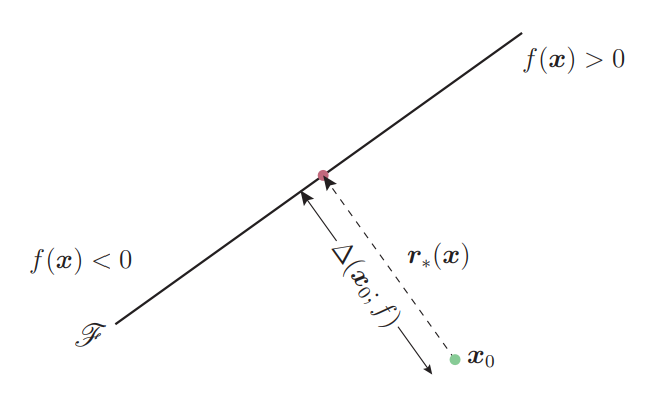
\includegraphics[width=0.49\textwidth]{img/other/deepfool_linear_binary.png}\label{fig:deepfool_1d}}
  \hfill
  \subfloat[Diferencijabilni binarni klasifikator. U svakom koraku se trenutnu točku aproksimira funkcija klasifikatora s hiperravninom i napravi projekcija na pravac koji siječe $\mathbb{R}^{n}$ (narančaste boje).]{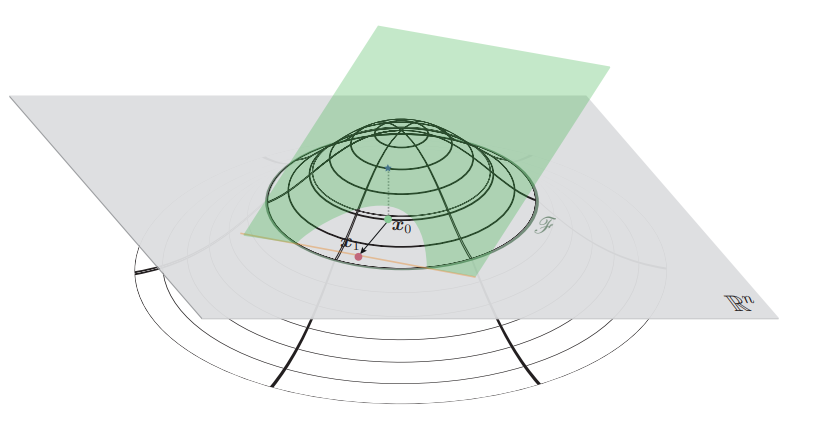
\includegraphics[width=0.49\textwidth]{img/other/deepfool_differential_binary.png}\label{fig:deepfool_2d}}
  \caption{Ilustracija rada DeepFool algoritma na binarnim klasifikatorima.}
\end{figure}\label{fig:deepfool_illustrations}

Pošto je i za rad ovog algoritma potrebo znanje o mreži, ovo je također napad na model bijele kutije. DeepFool pronalazi daleko bolje neprijateljske primjere s daleko manjim perturbacijama. Slijedi nekoliko primjera napada na ResNet50 mrežu.\\
slike


\chapter{Obrana dubokih konvolucijskih modela I}
Do sada je predstavljeno nekoliko napada. Originalni napad temeljen na minimizaciji približnog problema uz pomoć L-BFGS algoritam je opisan zbog povijesnih razloga. Napad nije u primjeni jer je u praksi vrlo spor i ne daje dobre rezultate. Međutim, pojavilo se mnoštvo potencijalnih obrana od dosadašnjih napada. U ovom poglavlju su opisane tri glavne kategorije takvih obrana na primjeru pojedinačnih obrana: 
\begin{enumerate}[noitemsep, label=\textbullet]
\item Jednostavne obrane -- konceptualno vrlo jednostavne za shvatiti, nije potrebno duboko predznanje o napadima, "jeftine" za implementirati
\item Neprijateljsko treniranje -- poboljšanje robustnosti klasifikatora još pri treniranju
\item Prikrivanje gradijenata -- vođeni idejom povećanja nelinearnosti mreže, određeni napadi namjerno ili slučajno "prikrivaju" gradijente mreže i time prividno sprječavaju napade temeljene na gradijentima
\end{enumerate}

\section{Jednostavne obrane}
U ovom dijelu je ukratko opisano nekoliko vrlo jednostavnih obrana. Dobra strana ovih obrana je što su iznimno jednostavne za implementirati i vrlo efektivne protiv već stvorenih neprijateljskih primjera, te nije potrebno nikakvo mijenjanje samog modela niti detaljno poznavanje potencijalnih metoda napada. Negativno je to što su pre-jednostavne da bi spriječile stvaranje novih neprijateljskih primjera te ne povećavaju robustnos mreže. Općenito, obrane koje su "agnostične" što se tiče modela kojeg brane, odnosno nezavisne su od modela, su u pravilu neuspješne.
\subsection{JPEG kompresija}
JPEG kompresija u obliku obrane od neprijateljskih primjera se pojavila više puta u različitim oblicima\citep{jpeg1}\citep{jpeg2}\citep{jpeg3}, a slijedi opis najjednostavnijeg načina zaštite. \\
JPEG je vrsta sažimanja podataka s gubitkom (eng. \textit{lossy}) za slike. Upravo to svojstvo je poželjno pri uništavanju neprijateljske perturbacije. Pretpostavka je da su i sami neprijateljski primjeri osjetljivi na perturbacije, odnosno da će male promjene nad pažljivo-konstruiranom perturbacijom vratiti sliku nazad u domenu ispravne klasifikacije. Ovo dodatno ima smisla kada se uzme u obzir da su neprijateljski primjeri rijetki, to jest da ih nije moguće lako nasumično pronaći. \\
JPEG kompresija bazira se na diskretnoj kosinusnoj transformaciji (eng. \textit{discrete cosine transform}, DCT). Transformacijom iz prostorne domene u frekvencijsku domenu omogućava se direktna manipulacija frekvencijskom domenom. Ljudski vid nije toliko osjetljiv na komponente visoke frekvencije u slikama, stoga se provodi kvantizacija frekvencija i visoke frekvencije se čuvaju s manjom preciznošću nego niske frekvencije. Preciznost pri kojoj se čuvaju visoke frekvenciji ovisi o faktoru kvalitete koji je u rasponu od $0$ do $100$: za $0$ se visoke frekvencije potpuno odbacuju, a za $100$ visoke frekvencije su maksimalno očuvane. Važno je uočiti da kvaliteta od $100$ ne znači da je kompresija bez gubitka, jer se gubitak djelomično dogodi već pri prelasku u frekvencijsku domenu. Na slici \ref{bla} se nalazi usporedba kompresije za različite kvalitete.
\par
Najjednostavnija verzija obrane (i prva koja se pojavila) je korištenje JPEG kompresije samo pri evaluciji. Autori su isprobali FGSM napad uz $\epsilon \in \{1, 5, 10\}$. Koraci su sljedeći:
\begin{enumerate}[noitemsep, label=\textbullet]
  \item izračunati neprijateljske primjere za navedene $\epsilon$
  \item provesti JPEG kompresiju nad običnim slikama i neprijateljskim primjerima
  \item usporediti izlaz modela za sve navedene skupove
\end{enumerate} \\

slike i grafovi možda \\

Zaključak je dakle da je jednostavna obrana temeljena na JPEG kompresiji daleko od korisnog rješenja, bar za FGM napad. Međutim DeepFool ima daleko manje peturbacije od FGSM napada, pa se isplati ponoviti i analizu za DeepFool. \\

slike i grafovi možda

\subsection{Gaussovo zaglađivanje / stiskanje značajki ?}

\section{Neprijateljsko treniranje - FGSM}
\section{Termometar kodiranje}

\chapter{Neprijateljski primjeri II}
\section{Neučinkovitost obrana} ...
\section{PGD} pgd\citep{Madry2017TowardsDL}
\section{Napadi \textit{Carlini and Wagner}} candw\citep{Carlini2017TowardsET}
\section{Napad temeljen na odluci} boundary\citep{Brendel2017DecisionBasedAA}

\chapter{Obrana dubokih konvolucijskih modela II}
\section{Preduvjeti uspješnih obrana}
\section{Neprijateljsko treniranje - PGD}
\subsection{FBF training}
\section{Dokazivost obrane od neprijateljskih napada}
\section{Budući rad}

\chapter{Zaključak}
Konvolucijske neuronske mreže su se pokazale iznimno uspješnima pri rješavanju problema klasifikacije slika. Međutim, pojava neprijateljskih primjera dovela je u pitanje tvrdnju da današnji modeli dobro generaliziraju. Također se ispostavilo da je vrlo lako osmisliti uspješne algoritme koji mogu generirati neprijateljske primjere, a za neke napade čak nije potrebno nikakvo dodatno znanje o mreži koju se napada. Ubrzo nakon pojave neprijateljskih primjera su se pojavile i prve potencijalne obrane. Iako su sve obrane na prvi pogled izgledale obećavajuće, pokazano je da većina tih obrana također ne mogu generalizirati na jače napade. Od svih obrana do sada, gotovo niti jedna obrana nije se pokazala korisnom. Najobećavajuća obrana do sada temelji se na posebnom obliku treniranja mreže korištenjem neprijateljskih primjera, no to je ono što tu obranu čini skupom i neuporabljivom na većim skupovima podataka kao što je \textit{ImageNet}. Budućnost obrana od neprijateljskih primjera još uvijek nije očita. Praktički svaki dan se pojavljuju sve efikasnije metode temeljene na suparničkom treniranju, formalni postupci koji mogu dokazati robustnost mreže te potpuno nove metode obrana koje će tek biti detaljno testirane. Međutim, danas obrana dubokih konvolucijskih modela još uvijek stoji kao vrlo izazovan i neriješen problem.


\bibliography{literatura}
\bibliographystyle{fer}

\chapter{Dodatak}\label{dodatak}
\section{Osobni skup slika}\label{osobni_skup}
U skupu slika \ref{ref_personal_image_table} je $16$ slika i labela koje su u radu korištene za generiranje suparničkih primjera za modele trenirane na \textit{ImageNet} skupu podataka. Sve slike su odabrane tako da spadaju unutar $1000$ razreda za koje su modeli predviđeni, dakle slike bi trebale biti ispravno klasficirane. Također, sve slike su unaprijed izrezane u oblik kvadrata kako ne bi došlo do prevelike degradacije kvalitete pri smanjenju rezolucije na $224\times224$. Ovim putem se zahvaljujem Sarah James na dopuštenju za korištenje slika u radu.

\section{Izlazi modela na nepromijenjenim slikama iz osobnog skupa}
Slike iz \ref{osobni_skup} su birane tako da budu reprezentativne, odnosno da ne postoji mogućnost da su mreže "zbunjene" oko toga što je na slici. Ideja iza toga je pokazati kako je neprijateljske primjere lako konstruirati čak i kada je mreža iznimno sigurna u to što vidi na slici. U tablici \ref{regular_predictions} nalaze se top-1 izlazi mreža \textit{ResNet50 V2} (primarna mreža korištena kroz rad) i \textit{Xception}.
\\
\bgroup
\def\arraystretch{1.2}
\begin{table}[H]
\begin{tabular}{|c | c | c|}
\hline
Slika & ResNet50 V2 & Xception \\ \hline
\ref{ref_pi01} & African grey $100.00\%$ & African grey $100.00\%$  \\ \hline
\ref{ref_pi02} & Backpack $99.71\%$ & Backpack $99.99\%$ \\ \hline
\ref{ref_pi03} & Dragonfly $99.93\%$ & Dragonfly $99.79\%$ \\ \hline
\ref{ref_pi04} & Bald eagle $87.47\%$ & Bald eagle $99.62\%$ \\  \hline
\ref{ref_pi05} & Grocery store $90.81\%$ & Grocery store $97.68\%$ \\ \hline
\ref{ref_pi06} & Gorilla $99.83\%$ & Gorilla $99.96\%$ \\ \hline
\ref{ref_pi07} & Guinea pig $100.00\%$ & Guinea pig $99.99\%$ \\ \hline
\ref{ref_pi08} & Jack-o'-lantern $100.00\%$ & Jack-o'-lantern $99.89\%$ \\ \hline
\ref{ref_pi09} & Jigsaw puzzle $100.00\%$ & Jigsaw puzzle $100.00\%$ \\ \hline
\ref{ref_pi10} & Computer keyboard $65.34\%$ & Computer keyboard $99.68\%$ \\ \hline
\ref{ref_pi11} & Llama $100.00\%$ & Llama $100.00\%$ \\ \hline
\ref{ref_pi12} & Meerket $99.98\%$ & Meerket $99.89\%$ \\ \hline
\ref{ref_pi13} & English Springer $88.93\%$ & English Springer $99.30\%$ \\ \hline
\ref{ref_pi14} & Running shoe $80.76\%$ & Running shoe $99.48\%$ \\ \hline
\ref{ref_pi15} & Tabby $64.28\%$ & Tabby $89.72\%$ \\ \hline
\ref{ref_pi16} & Wardrobe $87.16\%$ & Wardrobe $79.05\%$ \\ \hline
\end{tabular}
\caption{Tablica top-1 izlaza mreža ResNet50 V2 i Xception za slike iz \ref{osobni_skup}.}\label{regular_predictions}
\end{table}
\egroup

\begin{figure}[H]
    \centering
    % images 1-4
    \subfloat[\textit{African grey} (87)]{
        \label{ref_pi01}
        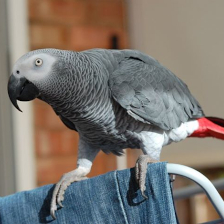
\includegraphics[width=0.25\textwidth]{img/personal_images/african_grey.jpg}
    }
    \subfloat[\textit{Backpack} (414)]{
        \label{ref_pi02}
        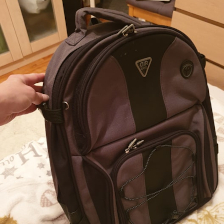
\includegraphics[width=0.25\textwidth]{img/personal_images/backpack.jpg}
    }
    \subfloat[\textit{Dragonfly} (319)]{
        \label{ref_pi03}
        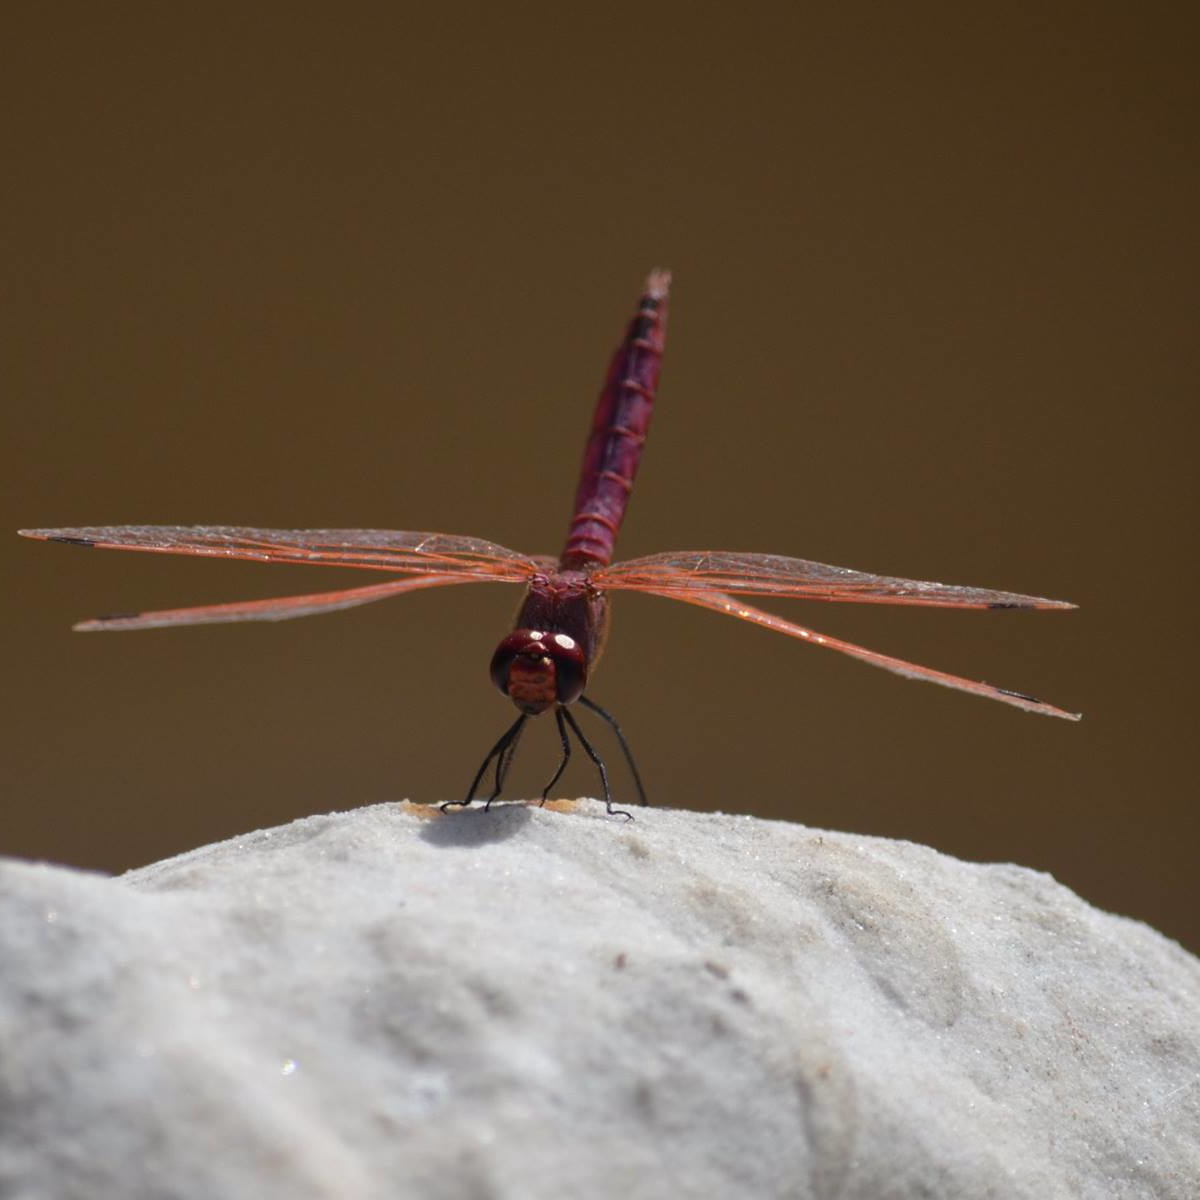
\includegraphics[width=0.25\textwidth]{img/personal_images/dragonfly.jpg}
    }
    \subfloat[\textit{Bald eagle} (22)]{
        \label{ref_pi04}
        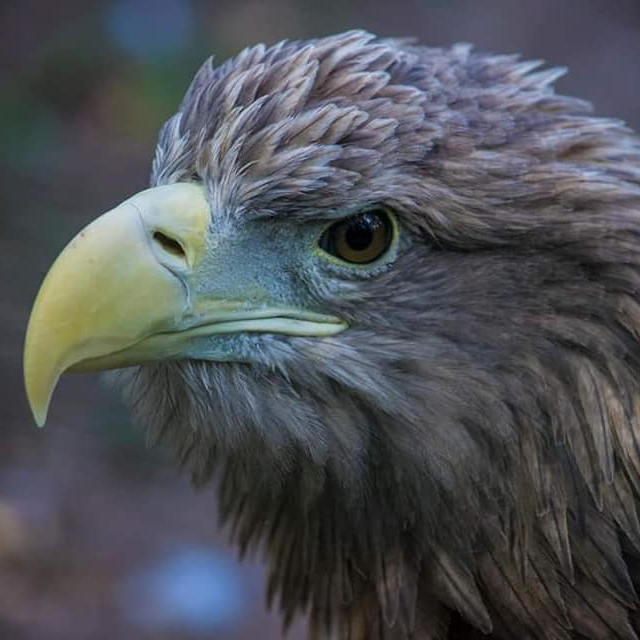
\includegraphics[width=0.25\textwidth]{img/personal_images/eagle.jpg}
    }
    \newline
    % images 5-8
    \subfloat[\textit{Grocery store} (582)]{
        \label{ref_pi05}
        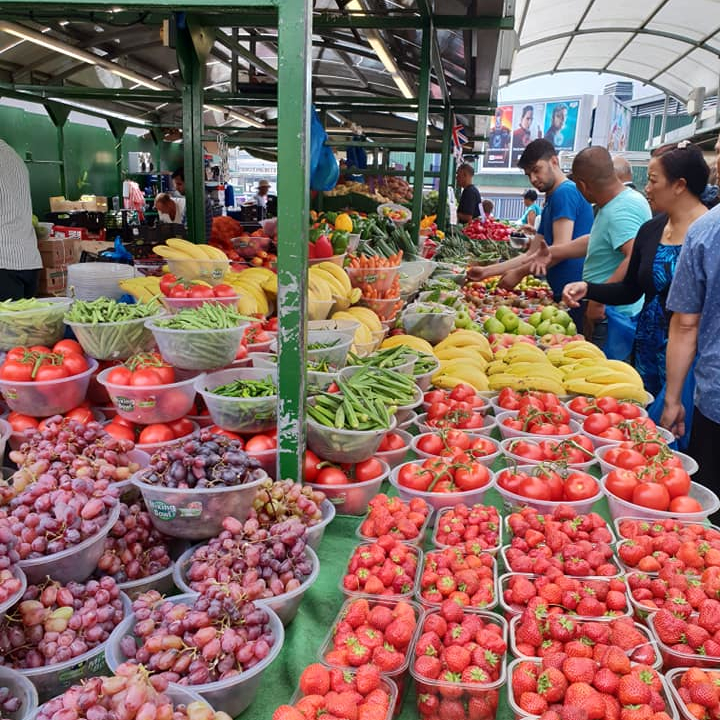
\includegraphics[width=0.25\textwidth]{img/personal_images/food_market.jpg}
    }
    \subfloat[\textit{Gorilla} (366)]{
        \label{ref_pi06}
        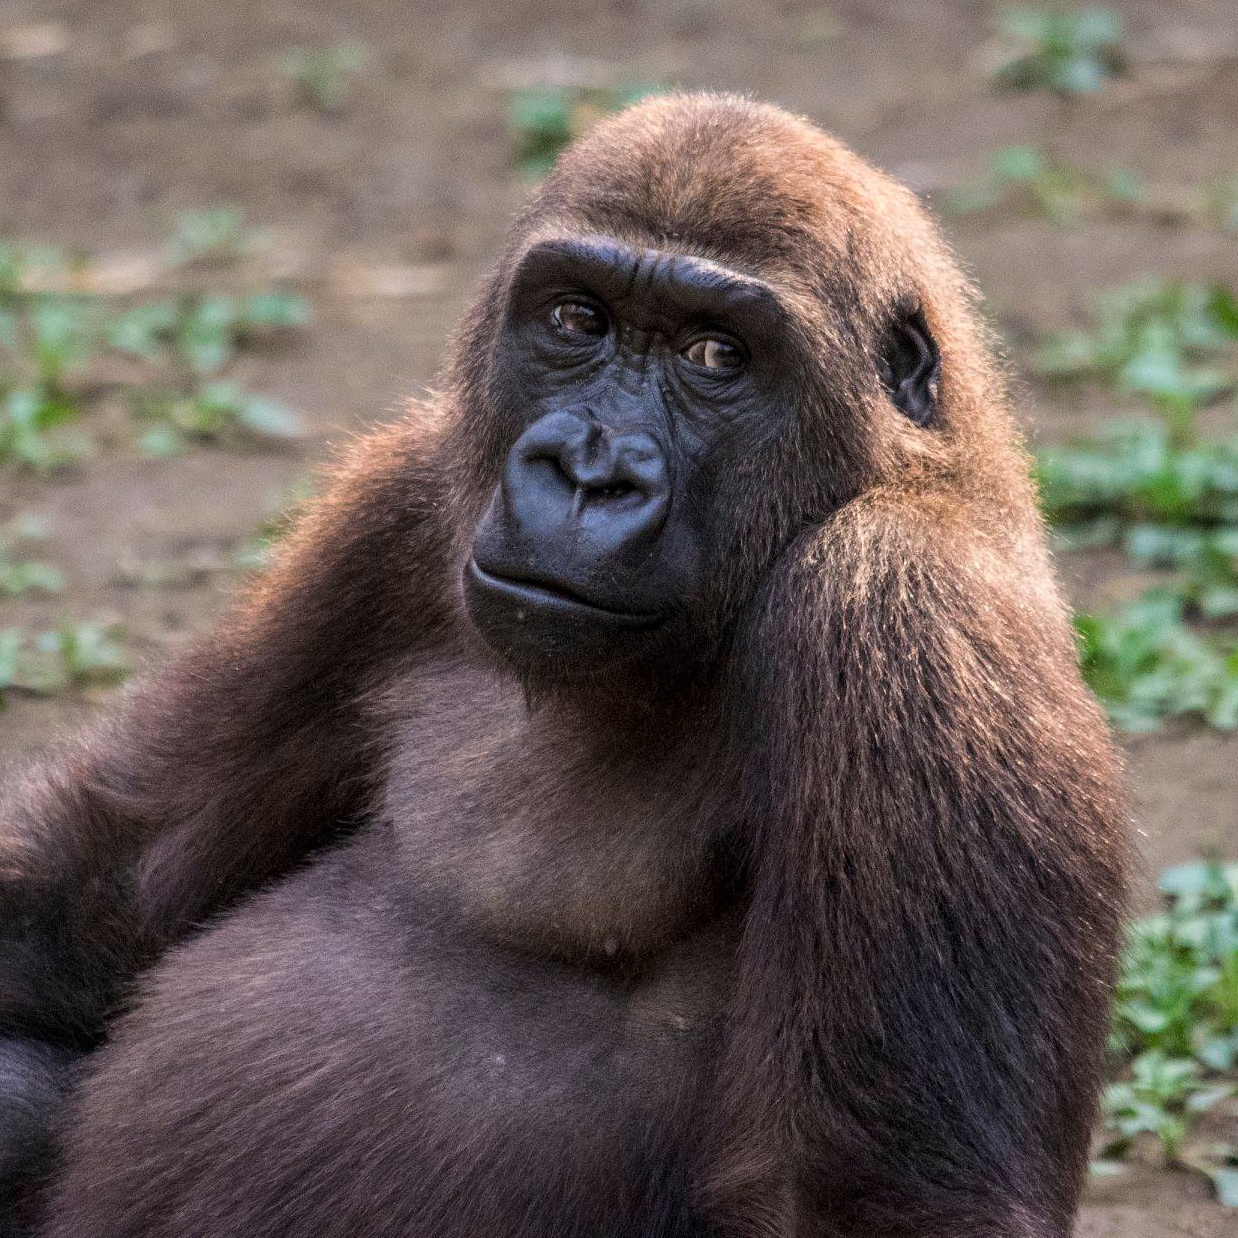
\includegraphics[width=0.25\textwidth]{img/personal_images/gorilla.jpg}
    }
    \subfloat[\textit{Guinea pig} (338)]{
        \label{ref_pi07}
        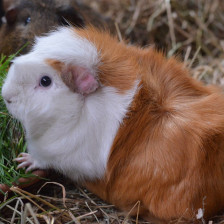
\includegraphics[width=0.25\textwidth]{img/personal_images/guinea_pig.jpg}
    }
    \subfloat[\textit{Jack-o'-lantern} (607)]{
        \label{ref_pi08}
        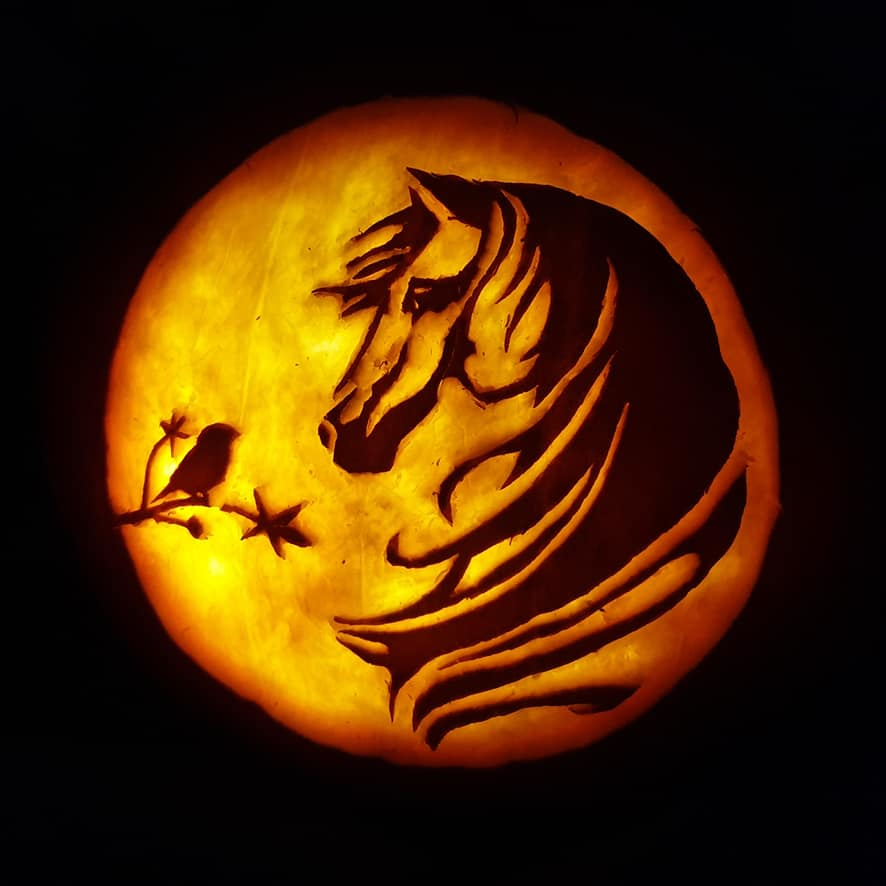
\includegraphics[width=0.25\textwidth]{img/personal_images/jackolantern.jpg}
    }
    \newline
    % images 9-12
    \subfloat[\textit{Jigsaw puzzle} (611)]{
        \label{ref_pi09}
        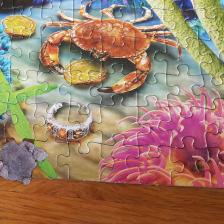
\includegraphics[width=0.25\textwidth]{img/personal_images/jigsaw2.jpg}
    }
    \subfloat[\textit{Keypad} (508)]{
        \label{ref_pi10}
        \includegraphics[width=0.25\textwidth]{img/personal_images/keyboard.jpg}
    }
    \subfloat[\textit{Llama} (355)]{
        \label{ref_pi11}
        \includegraphics[width=0.25\textwidth]{img/personal_images/llama.jpg}
    }
    \subfloat[\textit{Meerkat} (299)]{
        \label{ref_pi12}
        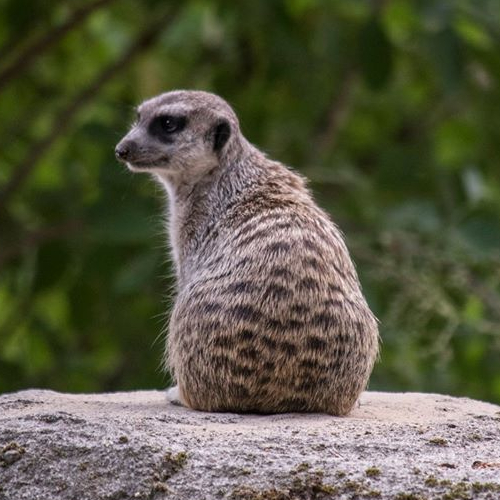
\includegraphics[width=0.25\textwidth]{img/personal_images/meerkat.jpg}
    }
    \newline
    % images 13-16
    \subfloat[\textit{English springer} \newline \centerline{(217)}]{
        \label{ref_pi13}
        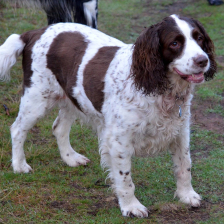
\includegraphics[width=0.25\textwidth]{img/personal_images/megan.jpg}
    }
    \subfloat[\textit{Running shoe} (770)]{
        \label{ref_pi14}
        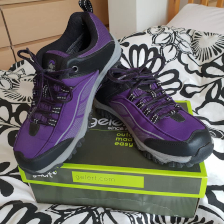
\includegraphics[width=0.25\textwidth]{img/personal_images/running_shoes.jpg}
    }
    \subfloat[\textit{Tabby} (281)]{
        \label{ref_pi15}
        \includegraphics[width=0.25\textwidth]{img/personal_images/tabby.jpg}
    }
    \subfloat[\textit{Wardrobe} (894)]{
        \label{ref_pi16}
        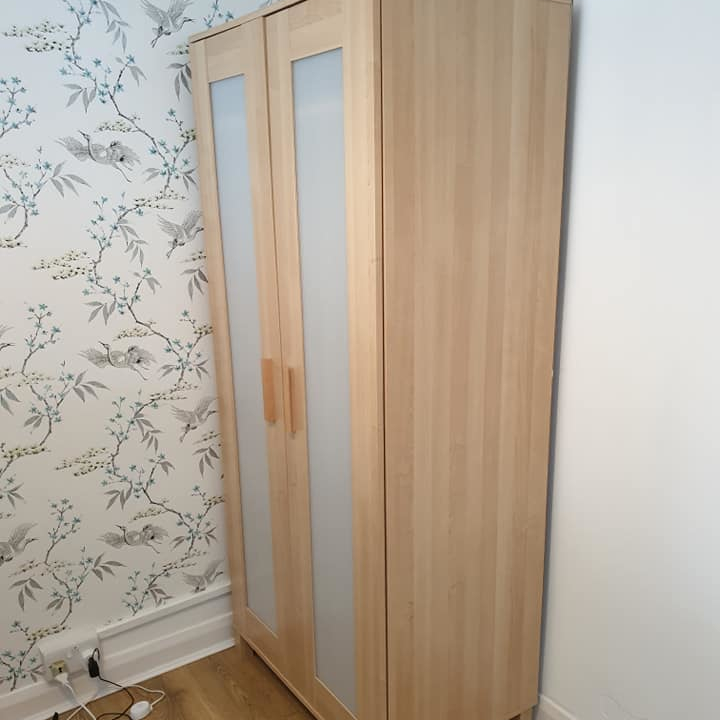
\includegraphics[width=0.25\textwidth]{img/personal_images/wardrobe.jpg}
    }
    
    \caption{Slike korištene za generiranje suparničkih primjera te njihove ispravne labele}
    \label{ref_personal_image_table}
\end{figure}


\begin{sazetak}
Današnji konvolucijski modeli postižu visoku točnost u području raspoznavanja objekata. Način rada dubokih modela je još uvijek vrlo teško ili nemoguće interpretirati, a dodatan razlog za brigu predstavljaju i takozvani neprijateljski primjeri. Neprijateljski primjeri su slike s dodanim teško uočljivim perturbacijama koje potiču model na pogrešnu klasifikaciju. Pokazalo se da je vrlo lagano konstruirati brze i efikasne napade na postojeće modele, nakon čega su se ubrzo pojavile i obrane protiv takvih napada. Nedugo nakon toga pojavljuju se sve jači napadi, dok su obrane stagnirale te danas još uvijek ne postoji zadovoljavajuća obrana protiv neprijateljksih napada. U radu je dan pregled spomenutih jednostavnih napada i jednostavnih obrana, istaknuta je neuspješnost jednostavnih obrana protiv jačih napada te je opisana obećavajuća obrana koja se temelji na treniranju mreže korištenjem neprijateljskih primjera.

\kljucnerijeci{klasifikacija objekata, konvolucijske neuronske mreže, računalni vid, suparnički primjeri, neprijateljski primjeri, obrana}
\end{sazetak}
\pagebreak
\engtitle{Defending Deep Convolutional Models from Adversarial Examples}
\begin{abstract}
Today's convolutional models can achieve high accuracy in the field of object recognition. The way deep models work is still very difficult or impossible to interpret, and an additional reason for concern are the so-called adversarial examples. Adversarial examples are images with added imperceptible perturbations that encourage the model to misclassify the image. It turned out to be very easy to construct fast and effective attacks on existing models, after which new defenses against these attacks also appeared. Soon afterwards even stronger attacks appeared, while new defenses stagnated and today there isn't a satisfactory defense against adversarial attacks. The thesis reviews the aforementioned simple attacks and simple defenses, pointing out the failure of simple defenses against strong attackers. Additionally, a promising defense is described. The defense is based on the concept of adversarial training and has shown good results.

\keywords{object classification, convolutional neural networks, computer vision, adversarial attacks, defense}
\end{abstract}
\end{document}
